%!TEX root = ../main.tex

\chapter{Data processing\label{chap:data_processing}}

The data has ben analyzed using Python in a Jupyter notebook
\footnote{Source code is available at: \url{https://github.com/kubakubakuba/mrs-uvdar-distance-estimator}},
with libraries from Metavision SDK\footnote{Metavision SDK Docs: \url{https://docs.prophesee.ai/stable/index.html}}.
The notebook if divided into sections that represent several datasets that were recorded during the measurements.
Precomputed average number of events with the standard deviation is stored in \texttt{.npz} files in the \texttt{./data} directory.

\section{Distance - frequency influence}

The distance frequency dataset has recordings of the UAV placed at 0 and 45 degrees relative to the event camera. This ensures data is captured from either
one LED source pointed directly at the event camera, or 2 LED sources pointed at the event camera at an angle. At each distance a new subdirectory was
created, with its name being the distance in meters and the content being the recordings of various frequencies in sequence, ordered by the recording timetamp.
With the range of frequencies\footnote{The frequencies represented in this list are the actual frequencies sent to the UVDAR unit. The preserved frequencies
are half of the values in this list - UVDAR interprets the frequency with a reference to the length of the sequence (2 for on/off).} and distances being

\begin{lstlisting}
frequencies_Hz = [10, 25, 50, 100, 250, 500, 1000, 2500, 5000, 10000, 20000, 30000]
distances_m = [1.0, 1.2, 1.4, 1.6, 1.8, 2.0, 2.2, 2.4, 2.6, 2.8, 3.0, 4.0, 5.0]
\end{lstlisting}

We can load the dataset stored in raw files into a matrix representing the distances and frequencies, then load a select amount of events from each file.
The data is then resampled to a 1D array by summing polarities over a select bin width
\footnote{The bin width should be adjusted appropriately, as the farther the event camera is from the source, the fewer events are generated.}.
Peaks in this signal are then analyzed by scipy's findpeaks function,
and the average amount of events with the standard deviation is calculated for each frequency and distance.

We can see the influence of distance and frequency on the average number of events on
\reffig{fig:dist} and \reffig{fig:freqs} respectively. The data shows a decreasing trend of the average number of events
with the increase of distance or frequency. The drop related to the distance can be explained by the perceived intensity
decrease of the light source with an increasing distance. With an increasing frequency, the camera is not able to capture
all the changes that are generated by the light source. On very high frequencies and distances, the camera is not able
to detect any real events at all, as there is more noise generated by the camera itself at this point. This can be observed
at \reffig{fig:dist_2} with the frequency of $30$ kHz at $3$ meters.

If we now select one frequency and try to fit it with a curve,
we can see that the data can be approximated with a polynomial or exponential function as shown on \reffig{fig:fit1}.
The best fit without being too complex is the inverse square law, which can be expressed as
\begin{equation}
	\text{intensity} \propto \frac{1}{\text{distance}^2}
\end{equation}
More complex functions could be used to fit the data, but it would rather tend to overfitting instead
of representing the data in a more general way. The inverse square law approximates the data relatively well.

\begin{figure}[htbp]
	\centering
	\subfloat[Influence of distance on the average number of events.] {
	  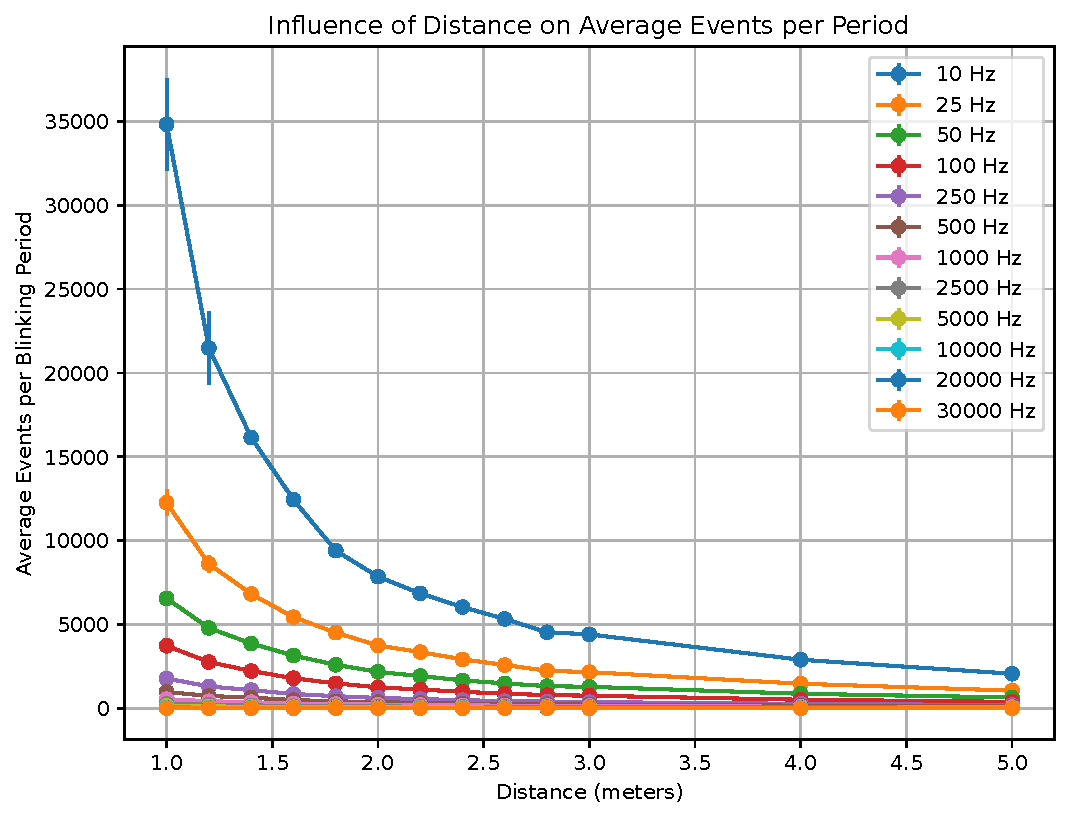
\includegraphics[width=0.5\textwidth]{./fig/plots/dist.pdf}
	  \label{fig:dist_1}
	}
	\subfloat[Influence of distance on the log of average number of events.] {
	  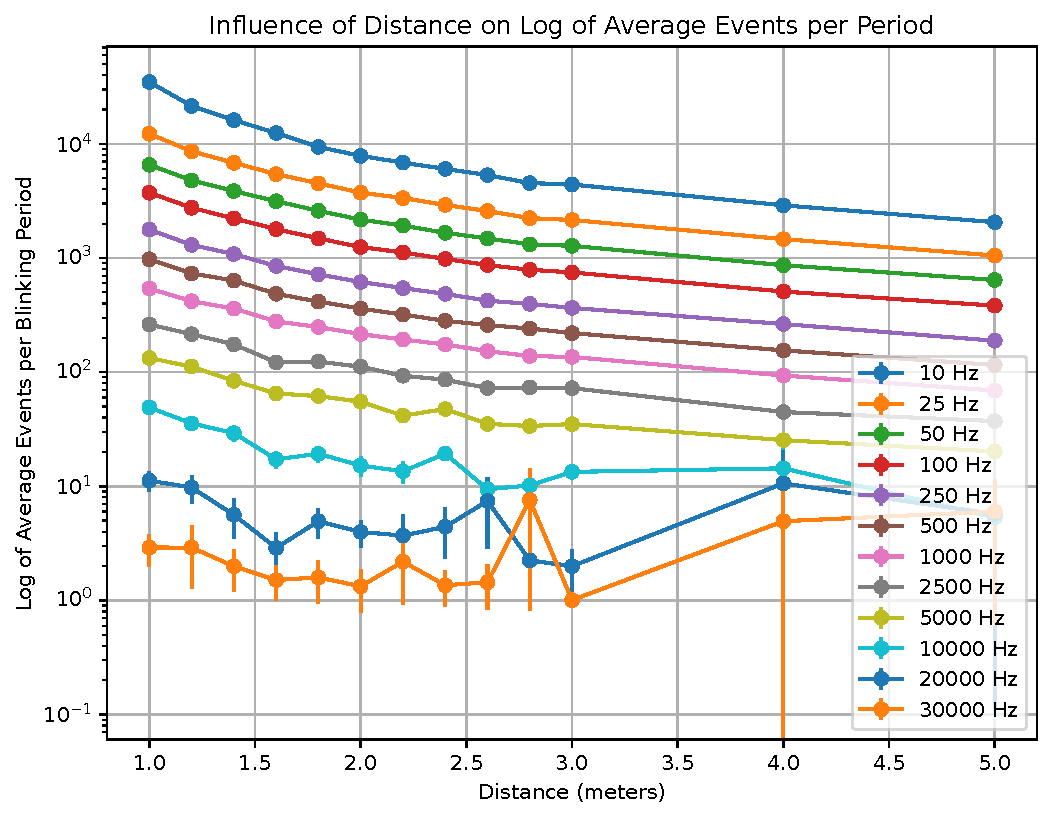
\includegraphics[width=0.5\textwidth]{./fig/plots/distlog.pdf}
	  \label{fig:dist_2}
	}
	\caption{
  The influence of distance on the average number of events with the UAV rotated 0 degrees relative to the event camera on \reffig{fig:dist_1}, and with the log of the average number of events on \reffig{fig:dist_2}.
  }
	\label{fig:dist}
\end{figure}

\begin{figure}[htbp]
	\centering
	\subfloat[Influence of frequency on the average number of events.] {
	  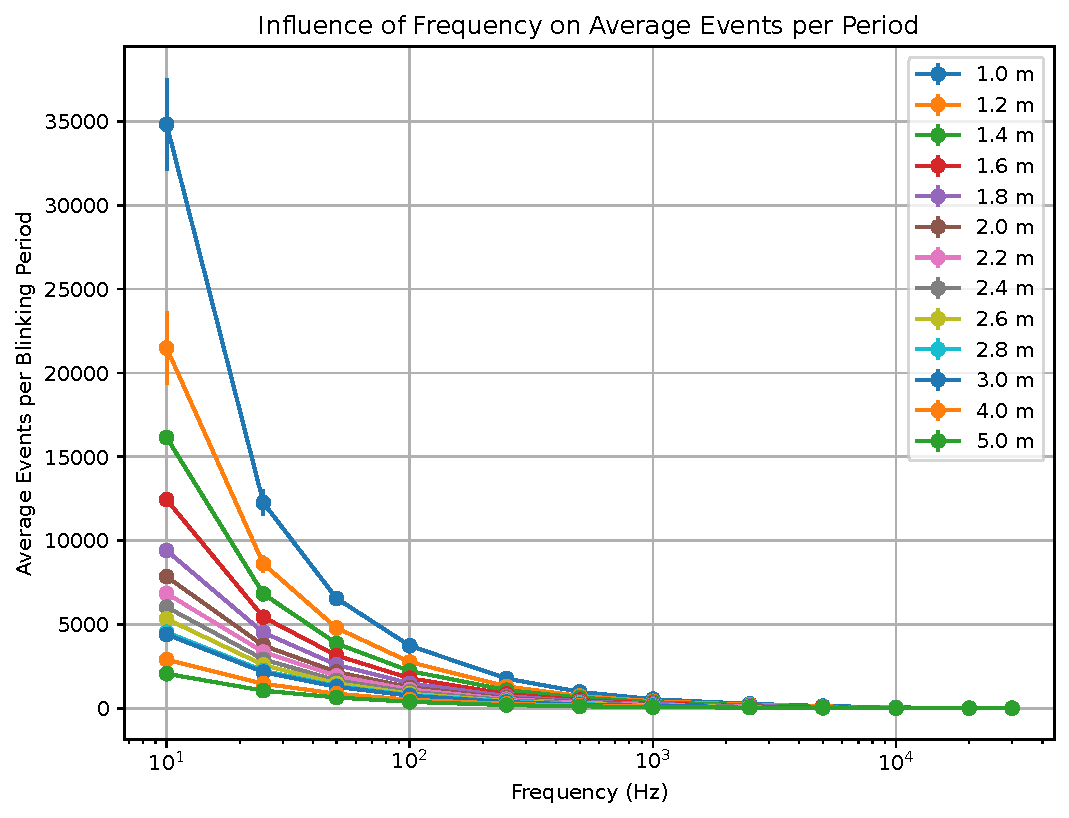
\includegraphics[width=0.5\textwidth]{./fig/plots/freqs.pdf}
	  \label{fig:freqs_1}
	}
	\subfloat[Influence of frequency on the log of average number of events.] {
	  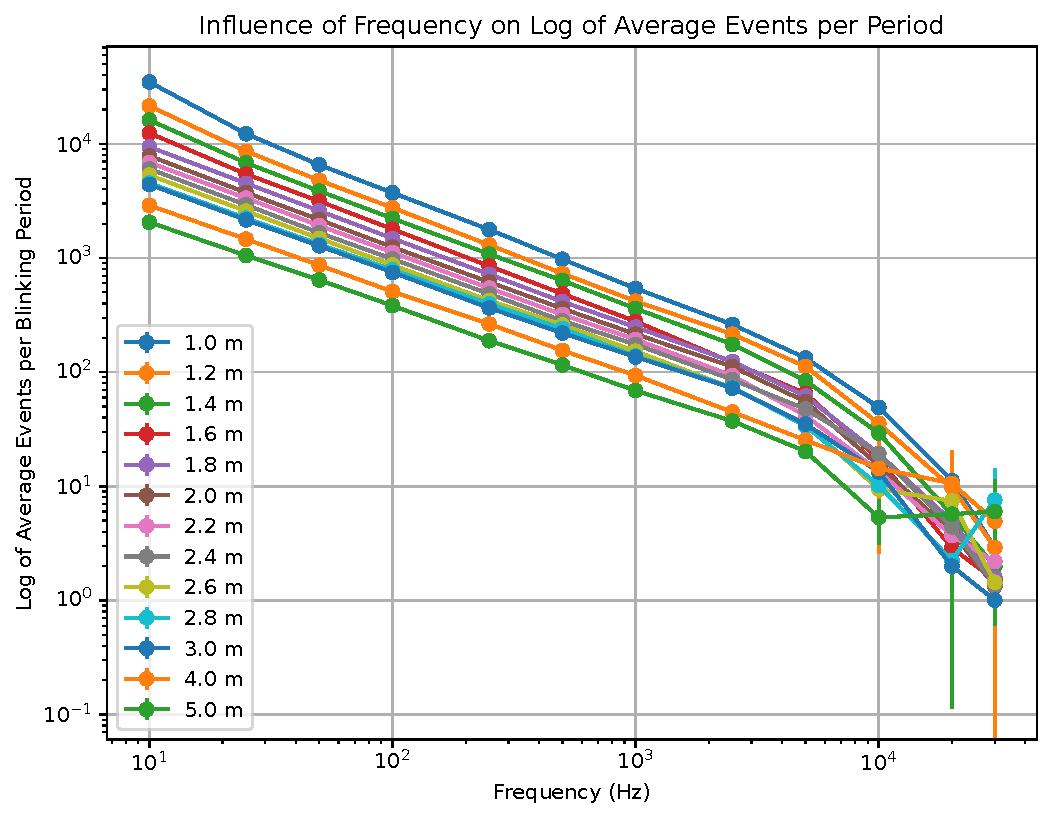
\includegraphics[width=0.5\textwidth]{./fig/plots/freqslog.pdf}
	  \label{fig:freqs_2}
	}
	\caption{
  The influence of frequency on the average number of events with the UAV rotated 0 degrees relative to the event camera on \reffig{fig:freqs_1}, and with the log of the average number of events on \reffig{fig:freqs_2}.
  }
	\label{fig:freqs}
\end{figure}

\begin{figure}[htbp]
	\centering
	\includegraphics[width=0.90\textwidth]{./fig/plots/inverse_square/square.pdf}
	\caption{Influence of distance data fitted with polynomial and exponential function.}
	\label{fig:fit1}
  \end{figure}

\newpage

\section{Rotation angle influence}

From the manufacturers datasheet for the UV LEDs\footnote{The datasheet of ProLight PM2B-1LLE 1W UV Power LED can be obtained from \url{https://www.tme.eu/Document/9dfb498784ffdd07892a42f4f17c6f37/PM2B-1LLE-DTE.pdf}}
used in the UVDAR system, we can learn that the LEDs have a lambertian radiation pattern,
which can be seen on \reffig{fig:lambertian}.
\begin {figure}[htbp]
	\centering
	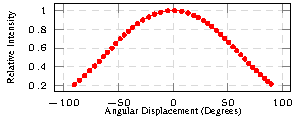
\includegraphics[width=0.75\textwidth]{./fig/plots/lambertian/lambertian.pdf}
	\caption{Lambertian radiation pattern of the UV LED.}
	\label{fig:lambertian}
\end{figure}

This means that the intensity of the light emmited from the LED decreases with the cosine
of the angle between the normal of the LED and the direction of the light \refeq{eq:lambertian}.
\begin{equation}
	I(\theta) = I_0\cos(\theta)
	\label{eq:lambertian}
\end{equation}
If we shift those distributions by $\pm 45$ degrees and sum them together, we can see the
theoretical distribution of the light emmited from the singular UAV arm \reffig{fig:lambert_combined}.
\begin {figure}[htbp]
	\centering
	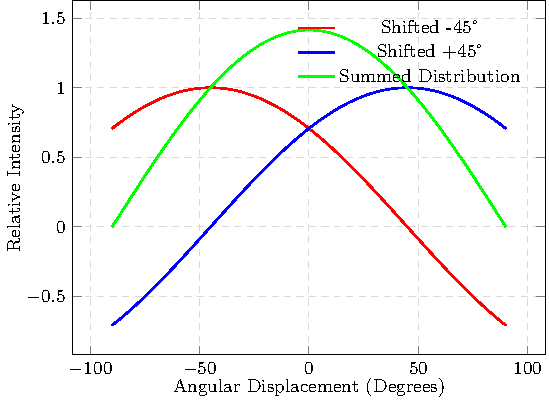
\includegraphics[width=0.75\textwidth]{./fig/plots/lambertian/3lambertian.pdf}
	\caption{Radiation pattern of two lambertian light sources shifted by $\pm 45$ degrees.}
	\label{fig:lambert_combined}
\end{figure}
With the dataset of the rotation of the UAV relative to the camera we will get the following results
on \reffig{fig:angles}.

\begin{figure}[htbp]
	\centering
	\subfloat[Influence of rotation of the UAV on the log of average number of events at 0.5 m.] {
	  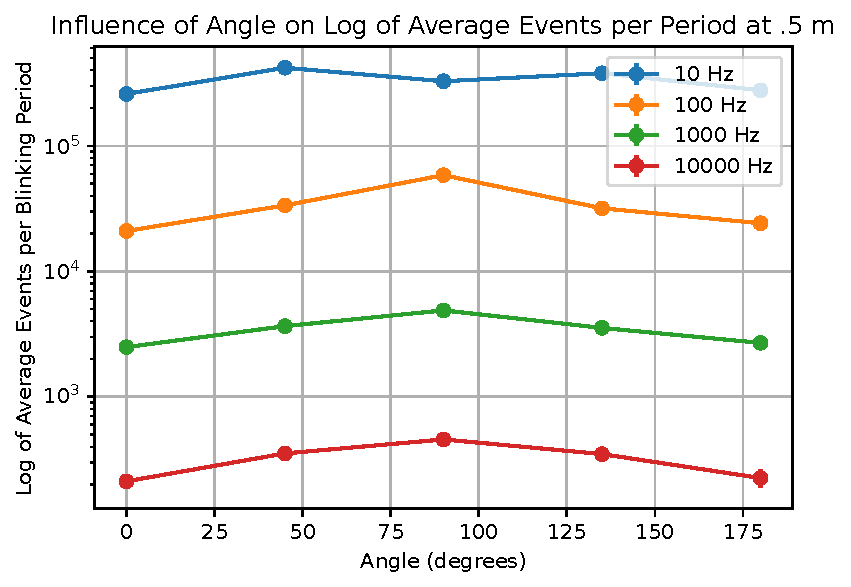
\includegraphics[width=0.5\textwidth]{./fig/plots/angle/angle1.pdf}
	  \label{fig:angle_1}
	}
	% \subfloat[Influence of rotation of the UAV on the log of average number of events at 1 m.] {
	%   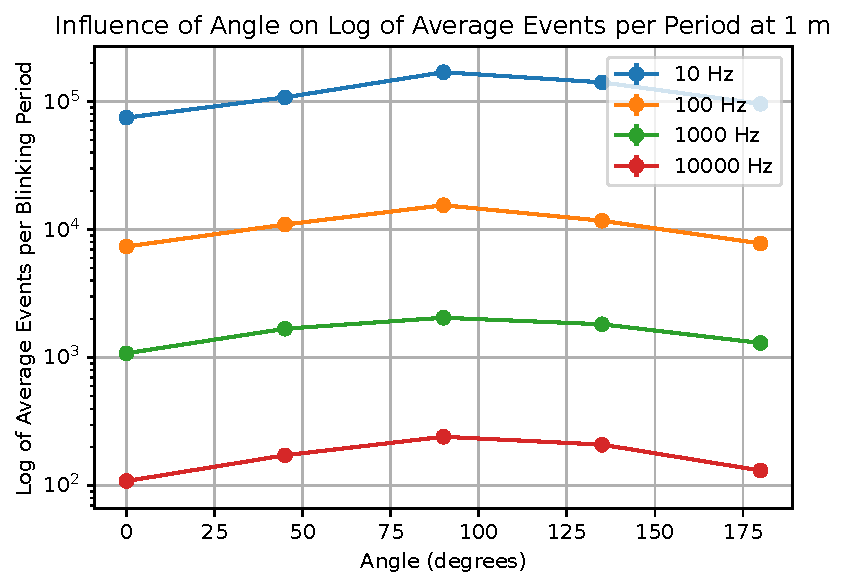
\includegraphics[width=0.5\textwidth]{./fig/plots/angle/angle2.pdf}
	%   \label{fig:angle_2}
	% }
	\subfloat[Influence of rotation of the UAV on the log of average number of events at 2 m.] {
	  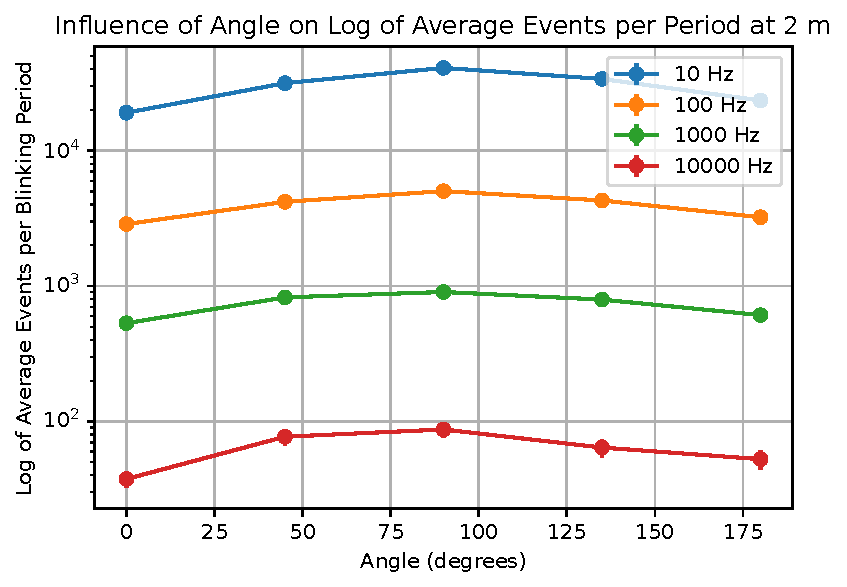
\includegraphics[width=0.5\textwidth]{./fig/plots/angle/angle3.pdf}
	  \label{fig:angle_3}
	}
	\caption{
  The influence of rotation angle on the log of average number of events at 0.5 m on \reffig{fig:angle_1} and at 2 m on \reffig{fig:angle_3}.
  }
	\label{fig:angles}
\end{figure}
The data shows a rough approximation of the theoretical distribution on \reffig{fig:lambert_combined},
but with a drop of intensity at the middle of the distribution. This could be caused
by the fact that the LEDs, when close to the camera, can be perceived as multiple light sources,
but when moved further away, they merge into one source as shown on \reffig{fig:leds}.

\begin{figure}[htbp]
	\centering
	\subfloat[2 LEDs with blinking frequency of 10 Hz at 0.5 m.] {
	  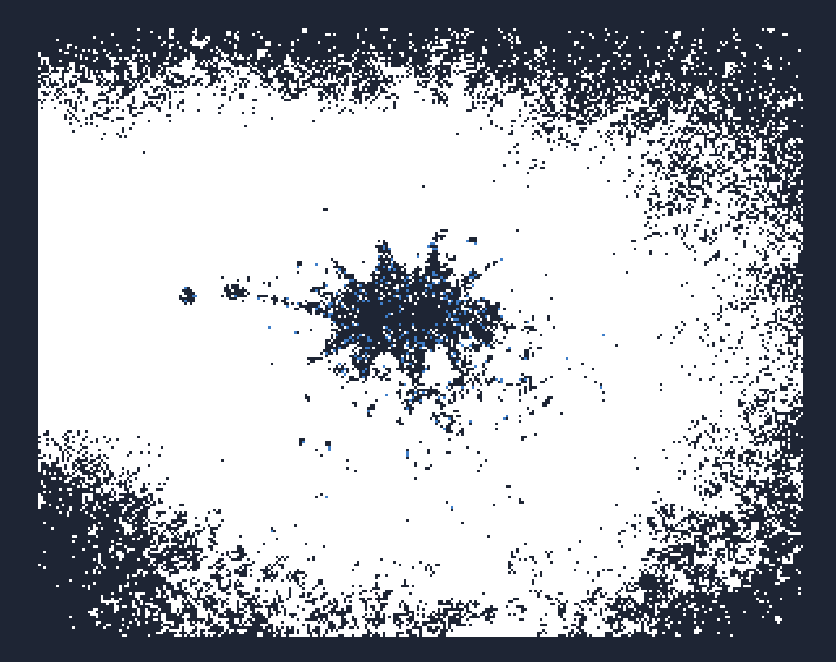
\includegraphics[width=0.5\textwidth]{./fig/photos/2leds_05m.png}
	  \label{fig:leds_1}
	}
	\subfloat[2 LEDs with blinking frequency of 10 Hz at 2 m.] {
	  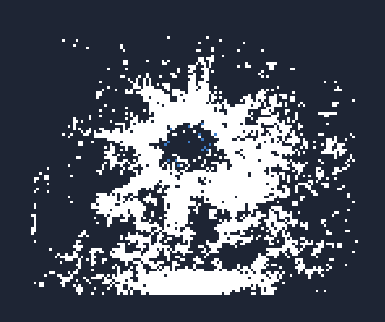
\includegraphics[width=0.5\textwidth]{./fig/photos/2leds_2m.png}
	  \label{fig:leds_2}
	}
	\caption{
  The light source on one arm of the UAV, consisting of two UV LEDs, blinking at a frequency of 10 Hz,
  placed at 0.5 m on \reffig{fig:leds_1} and 2 m at \reffig{fig:leds_2}.
  }
	\label{fig:leds}
\end{figure}
What we can also observe from \reffig{fig:leds} are the star-like shapes of the LEDs, which are supposed to be circular.
Those shapes are caused by light diffraction, which is caused by the aperture blades in the lens of the camera. The number
of star spikes depend on the number of blades, the set aperture and the light source intensity then causes stars of different
levels of profoundness.\cite{bhphoto2025star} We can observe this by comparing how profound are the star shapes on different
frequencies, as shown on \reffig{fig:stars}.

\begin{figure}[htbp]
	\centering
	\subfloat[LED blinking at 10 Hz at 1.0 m] {
	  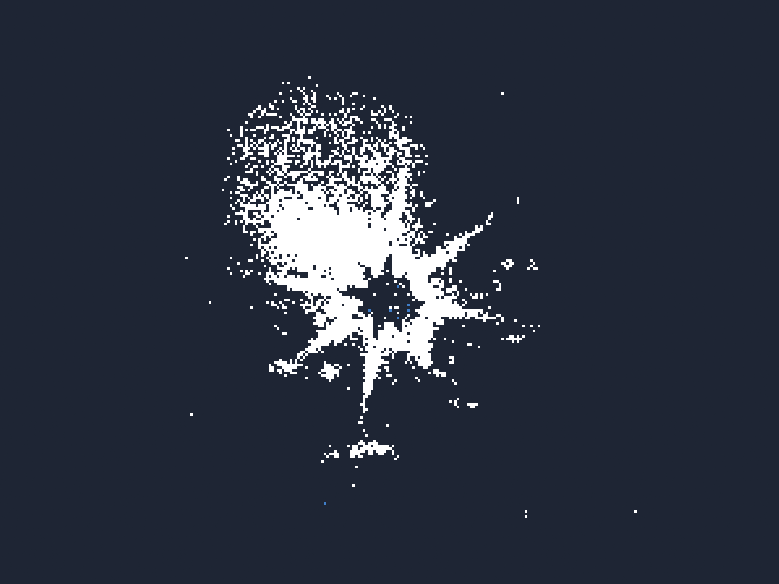
\includegraphics[width=0.5\textwidth]{./fig/photos/led_10hz.png}
	  \label{fig:stars_1}
	}
	\subfloat[LED blinking at 1 kHz at 1.0 m] {
	  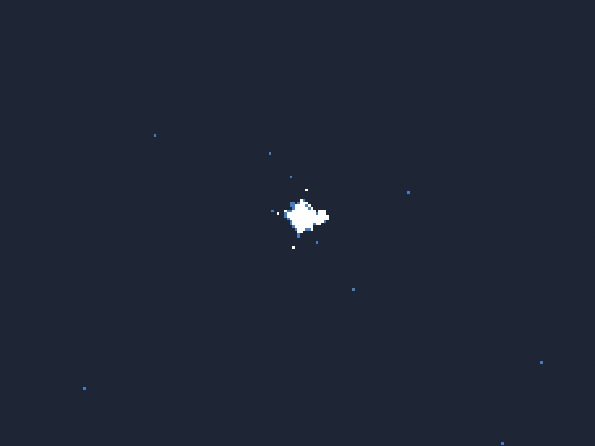
\includegraphics[width=0.5\textwidth]{./fig/photos/led_1000hz.png}
	  \label{fig:stars_2}
	}
	\caption{
  Two same LED light sources at 1.0 meters, blinking at 10 Hz and 1 kHz.
  \reffig{fig:stars_1} shows a visible diffraction star (while being much brighter), while \reffig{fig:stars_2} shows a
  much more cicular source of light that is not as bright.
  }
	\label{fig:stars}
\end{figure}